\documentclass{article}
\usepackage[T1]{fontenc}
\usepackage[utf8]{inputenc}
\usepackage[french]{babel}
\usepackage{enumitem}
\usepackage{amsmath}
\usepackage{amssymb}
\usepackage{graphicx}
\usepackage{listings}
\usepackage{hyperref}
\usepackage[dvipsnames]{xcolor}
\setcounter{tocdepth}{2}
\hypersetup{
    colorlinks,
    citecolor=black,
    filecolor=black, 
    linkcolor=black,
    urlcolor=black
}

\lstset{language=Python,
        basicstyle=\ttfamily,
        keywordstyle=\color{BlueViolet}\ttfamily,
        commentstyle=\color{OliveGreen}\ttfamily,
        breaklines=true,
}

\title{Rapport du devoir maison de Sécurité}
\author{BASUALDO Lautaro et LOI Léo}

\begin{document}
\maketitle

\tableofcontents
\newpage

\section{Exercice 1 :}

    Avant de pouvoir décrypter les deux mots de passes, nous devons déjà les identifier.\\
    Or, nous savons que la fonction SHA-256 génèrera toujours le même haché pour un mot de passe donné.\\
    Ainsi, nous pouvons détecter deux hachés différents :
    \begin{itemize}
        \item 068be8be83f9bfafd1545d357fd3cd132f8c659effd11e635a698811b796c880\\
        (utilisé par Bart, Homer, Lisa et March)
        \item 15e2b0d3c33891ebb0f1ef609ec419420c20e320ce94c65fbc8c3312448eb225\\
        (utilisé par Bob, Carlton, John et William)
    \end{itemize}

    Pour le premier haché, grâce aux différents indices, nous pouvons deviner que le mot de passe utilisé est le 74ème élément du tableau périodique des élements. A savoir le "tungstène" appelé en anglais "tungsten"\\
    Afin de s'assurer de nos résultats, nous avons haché le mot "tungsten" avec la fonction de hachage SHA-256 ce qui donne le résultat suivant :\\
    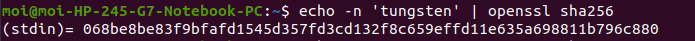
\includegraphics[scale = 0.5]{tungsten.png}
    Nous pouvons constater que les deux hachés sont similaire, le mot de passe utilisé par Bart, Homer, Lisa et March est donc bien "tungsten"\medskip

    Pour le second haché, grâce aux différents indices, nous pouvons deviner que le mot de passe utilisé est la suite de chiffres "123456789"\\
    Afin de s'assurer de nos résultats, nous avons haché le mot "123456789" avec la fonction de hachage SHA-256 ce qui donne le résultat suivant :\\
    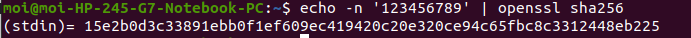
\includegraphics[scale = 0.5]{chiffre.png}
    Nous pouvons constater que les deux hachés sont similaire, le mot de passe utilisé par Bob, Carlton, John et William est donc bien "123456789"
\newpage
\section{Exercice 2 :}
    \subsection{Question 1 :}
        \lstinputlisting[linerange={8-46}]{ui.py}
    \subsection{Question 2 :}
        Après plusieurs éxecutions du programme ci-dessus, les valeurs suivantes peuvent être récupérées dans la base de donnée\newline
        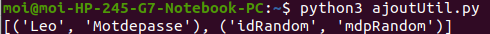
\includegraphics[scale = 0.5]{ajoutUtil.png}
    \subsection{Question 3 :}
        \lstinputlisting[linerange={54-67}]{ui.py}
    \subsection{Question 4 :}
        Notre fonction d'AjoutUtilisateur renvoyant une liste contenant l'identifiant et le mot de passe de l'utilisateur,
        il nous suffit de récupérer ces données, et de les renvoyer une fois le mot de passe haché
        \lstinputlisting[linerange={74-79}]{ui.py}
    \subsection{Question 5 :}
        \lstinputlisting[linerange={82-87}]{ui.py}
    \subsection{Question 6 :}
        \lstinputlisting[linerange={89-98}]{ui.py}
\newpage
\section{Exercice 3 :}


        


\end{document}